\documentclass[multip]{SGGW-thesis}
\title{Implementacja sieciowej gry wideo z wykorzystaniem silnika Unreal Engine 4}
\author{Maciej Wygoda}
\date{2017}
\university{Szkoła Główna Gospodarstwa Wiejskiego\\w Warszawie}
\dep{Wydział Zastosowań Informatyki i Matematyki}
\Etitle{Implementation of an online video game using Unreal Engine 4}
\album{172407}
\thesis{Praca dyplomowa inżynierska}
\course{Informatyka}
\promotor{dr. Bartłomieja Kubicy}
\pworkplace{Wydział Zastosowań Informatyki i Matematyki\\Katedra Zastosowań Informatyki}

%obrazki
\usepackage{graphicx}
\usepackage{enumitem}
%\usepackage{hyperref}
%https://tex.stackexchange.com/a/3034
\PassOptionsToPackage{hyphens}{url}\usepackage{hyperref}
%https://tex.stackexchange.com/questions/28333/continuous-v-per-chapter-section-numbering-of-figures-tables-and-other-docume
\usepackage{chngcntr}
\counterwithout{figure}{chapter}

\begin{document}
\maketitle
\twoppage{Maciej Wygoda}{172407}{ktore rodzialy + strony}{Marcin Szadkowski}{wpisz swoj numer albumu}{ktore rodzialy + strony}
\statementpage
\abstractpage
{Implementacja sieciowej gry wideo z wykorzystaniem silnika Unreal Engine 4}
{Niniejsza praca jest opisem implementacji sieciowej gry wideo z wykorzystaniem silnika Unreal Engine 4. Zawiera opis silnika, procesu projektowania i implementowania gry, prezentuje jej architekturę oraz zastosowane rozwiązania.}
{Unreal Engine 4, tworzenie gier wideo, gamedev, gra wideo}
{Implementation of an online video game using Unreal Engine 4}
{This study is a description of an implementation of an online video game using Unreal Engine 4. It describes the engine, the processes of designing and implementing the game and also presents the game's architecture and applied solutions.}
{Unreal Engine 4, game development, gamedev, video game}

\tableofcontents

\chapter{Wstęp}
Gry wideo stanowią rozrywkę dla coraz szerszego grona odbiorców, a sama branża nieustannie rośnie, o czym najlepiej świadczy fakt, iż pod względem wygenerowanych przychodów prześcignęła już branże filmową oraz muzyczną~\cite{nasdaq-video-games-industry}. Gry coraz częściej postrzegane są jako nowoczesne medium przekazu oraz forma wyrazu artystycznego i poruszają tematy dotychczas zarezerwowane dla literatury i kinematografii. 
\newline Tworzenie gier wideo ({\em ang. game development}) to obszerne zagadnienie łączące w sobie wiele dziedzin. Od strony technicznej są to między innymi grafika komputerowa, inżynieria oprogramowania, programowanie komputerów, bezpieczeństwo komputerowe, matematyka. W związku z tym, że stworzenie gry to proces długi i skomplikowany, istnieje wiele narzędzi wspierających go, a jednym z najpopularniejszych jest silnik {\em Unreal Engine 4} (zwany dalej "UE4").
\section{Cel i zakres pracy}
Głównym celem niniejszej pracy jest rozwój wiedzy o procesie tworzenia gier wideo. Ponadto motywację stanowiły chęć zgłębienia technologii UE4, podjęcia technicznego wyzwania, jakie stawia zaprogramowanie gry wideo oraz pasja do gier. Na całą pracę składa się zaprojektowanie i zaimplementowanie gry z użyciem UE4 oraz podstawowy opis silnika i implementacji gry. 
\newline Uwagę skupiono między innymi na poznawaniu działania i efektywnym wykorzystywaniu technologii UE4 oraz oprogramowania do modelowania i animacji Blender oraz zdobyciu doświadczenia w pracy zespołowej.
% oraz opracowaniu metodyki pracy, która pozwoli na wielokrotne wykorzystanie napisanego kodu oraz skrócenie czasu tworzenia oprogramowania.
\newline Praca ta może z powodzeniem służyć za przykład i drogowskaz dla osób chcących napisać własną grę.

\chapter{Unreal Engine 4}
\section{Czym jest silnik gry?}
Przez pojęcie ,,silnik gry`` rozumie się zbiór funkcji i narzędzi ({\em ang. framework}) wspierający tworzenie gier. Musi on oferować przede wszystkim renderowanie grafiki, dźwięku i obsługę sterowania aczkolwiek obecnie najpopularniejsze silniki posiadają znacznie więcej funkcji, a są to między innymi obsługa sieci, symulacja fizyki, edytory shaderów i efektów cząsteczkowych, produkcja przerywników filmowych oraz obsługa wielu platform na przykład komputerów, konsol czy urządzeń mobilnych takich jak smartfony. Każdy popularny silnik dystrybuowany jest wraz z edytorem będacym graficznym interfejsem między programistą, a funkcjami silnika.
\newline Wykorzystanie jednego silnika do stworzenia wielu różnych gier znacząco skraca okres produkcji i stanowi powszechną w branży praktykę.\cite{learning-unreal}\cite{wiki-game-engine}

\section{Funkcje silnika Unreal Engine 4}
%tu chodzi o ficzery unreala, info m.in. z naszej prezentacji na seminarium oraz
%\newline\url{https://www.unrealengine.com/en-US/features}
%\newline\url{https://docs.unrealengine.com/latest/INT/Engine/index.html}
UE4 swoją popularność zawdzięcza między innymi otwartemu źródłu, co w pewnym stopniu umożliwia producentom gier dostosowanie silnika do własnych potrzeb na przykład poprzez programowanie narzędzi dla mniej technicznych członków zespołu czy modyfikacje w działaniu silnika. Ponadto UE4 jest w stanie renderować grafikę bardzo zbliżoną do fotorealizmu, co w połączeniu z szeroką gamą oferowanych funkcji sprawia, że poza grami korzysta się z niego na przykład do produkcji spotów i aplikacji reklamowych. \cite{the-human-race}\cite{ikea-vr}
\newline
\newline Oprócz podstawowych funkcji takich jak renderowanie grafiki czy obsługa sterowania do dyspozycji oddane zostały między innymi \cite{docs-ue4-features}:
\begin{description}
\item[Symulacja fizyki:]UE4 korzysta z silnika fizyki {\em PhysX 3.3} dzięki czemu wiarygodnie symuluje kolizje obiektów i inne oddziaływania fizyczne. Producenci mają również możliwość modyfikowania panujących zasad celem lepszego przedstawienia własnej wizji.
\item[Edytor interfejsu użytkownika:] Interfejs stanowi istotny element w komunikacji między grą, a grającym. UE4 zapewnia rozbudowany edytor pozwalający na tworzenie między innymi takich elementów interfejsu jak {\em HUD (head-up display)} czy menu.
\item[Drzewa behawioralne:]Stanowią one podstawę sztucznej inteligencji w UE4 i pozwalają na zaprogramowanie zachowania postaci sterowanych przez komputer w zależności od odbieranych przez nie bodźców i stanu sceny.
\clearpage \item[Sequencer:]Jest to narzędzie służące do produkcji przerywników filmowych. Jego obsługa przypomina pracę z oprogramowaniem do montażu filmów i modelowania 3D. Edytor ten uwzględnia elementy takie jak oś czasu, ujęcia kamery, szkielety i animacje obiektów.
\item[Networking:]UE4 powstał z myślą o rozgrywce sieciowej, wobec tego dużo uwagi poświęcono stworzeniu odpowiedniej abstrakcji ułatwiającej programowanie komunikacji sieciowej. Komunikacja ta wykorzystuje model klient-serwer co oznacza, że istnieje jeden serwer z autorytatywną instancją świata oraz wielu klientów, których światy są aktualizowane na podstawie tego, co dzieje się na serwerze. Aktualizacje te opierają się o aktualizacje właściwości obiektów i zdalne wywołania procedur {\em (ang. remote procedure calls - RPC)}. W obu przypadkach wykorzystywany jest protokół {\em UDP}, który jest zawodny, ale generuje o wiele mniejszy narzut na sieć niż w przypadku {\em TCP}. UE4 ma zaimplementowany własny system zapewniający częściową niezawodność komunikacji. \cite{unreal-wiki-replication}
%https://docs.unrealengine.com/latest/INT/Gameplay/Networking/index.html
\item[Analiza wydajności:]Osiągnięcie iluzji ruchomego obrazu wymaga wygenerowania przynajmniej 15 klatek na sekundę ({\em ang. frames per second - FPS}), obecnie na konsolach do gier pożądaną wartością jest przynajmniej 30FPS, na komputerach 60FPS, a w tytułach esportowych nawet dwa razy więcej. Miara ta jest odzwierciedleniem płynności obrazu i wydajności gry, a na wydajność składają się stopień skomplikowania scen i obliczeń oraz optymalizacja. UE4 zapewnia narzędzia do profilowania, dzięki którym łatwiejsze staje się zidentyfikowanie obszarów wymagających optymalizacji.
\item[Edytor materiałów:]W konwencji UE4 materiał to zbiór informacji o wizualnej stronie obiektu. Do pewnego stopnia można o nim myśleć jak o farbie. Należy jednak uwzględnić, że materiał poza kolorem czy teksturą definiuje również rodzaj powierzchni obiektu (na przykład metal, drewno), przezroczystość i inne cechy, które mogą mieć wpływ na zachowanie światła padającego na dany obiekt. UE4 posiada rozbudowany edytor materiałów opierający się na programowaniu graficznym ({\em ang. visual scripting}).
\item[Blueprints Visual Scripting:]Jest to system graficznego programowania rozgrywki oparty o węzły reprezentujące elementy takie jak funkcje, klasy czy zmienne, które po połączeniu stanowią pewną logikę (rys. \ref{fig-bp-example}). Za pomocą blueprintów można (często w krótszym czasie) osiągnąć podobny efekt co za pomocą kodu przy czym dla osób mniej technicznych są one o wiele prostsze w użyciu. Ponadto mogą dziedziczyć klasy napisane kodem, a programiści mają możliwość rozwijania blueprintów poprzez programowanie kolejnych węzłów do użycia przez resztę zespołu. Jest możliwe napisanie kompletnej gry bez nawet jednej linii kodu, a jedynie z użyciem blueprintów. Nie oznacza to jednak, że kod stał się bezużyteczny. W każdym wypadku kod {\em C++} jest wydajniejszy od blueprintów (to znaczy szybciej się wykonuje, co bezpośrednio wpływa na liczbę generowanych klatek na sekundę), w wielu przypadkach jest czytelniejszy (na przykład obliczenia w pętli) i łatwiejszy w utrzymaniu (na przykład kontrola wersji przy pracy zespołowej).\cite{docs-blueprints}
\newline Oba te podejścia są wykorzystywane w profesjonalnym środowisku, a kluczem do sukcesu jest ich umiejętne połączenie, co zaprezentowano w dalszej części tej pracy.
\begin{figure}
	\centering
		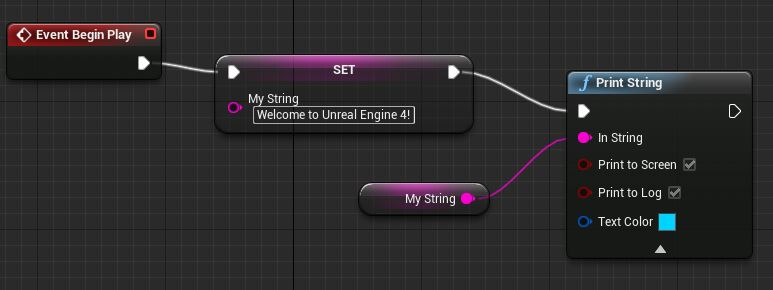
\includegraphics[width=1\textwidth]{figures/bp_example.jpg}
	\caption{Przykład blueprinta}
	\label{fig-bp-example}
\end{figure}

\end{description}

\section{Konwencja i architektura rozgrywki}
\label{sec:konwencja}
%\url{https://docs.unrealengine.com/latest/INT/Gameplay/Framework/index.html}
%\newline\url{https://docs.unrealengine.com/latest/INT/Gameplay/Framework/QuickReference/index.html}
%\newline obowiazkowo obrazek z dolu strony :D
Styl rozgrywki zależy od gry i wizji jej autora, jednak istnieją pewne cechy wspólne widoczne w niemal każdym tytule. Jest to na przykład sterowanie za pomocą urządzeń wejścia czy pewien zbiór zasad gry. Z tego powodu w UE4 przyjęto zaprezentowaną poniżej konwencję dotyczącą rozgrywki (rys. \ref{fig-gameplay-chart}).\cite{docs-gameplay-framework}
\begin{description}
\item[Actor:]Jest to bazowa klasa dla każego obiektu, który można umieścić w scenie. Obiekty te nie muszą mieć fizycznej reprezentacji. Często zawierają dodatkowe komponenty ~({\em ActorComponents}) określające między innymi w jaki sposób obiekt się porusza czy jak jest renderowany. Oprócz tego {\em aktor} posiada obsługę replikacji właściwości i wywołań funkcji przez sieć.
\item[Pawn:]Jest to {\em aktor}, który może być kontrolowany przez gracza lub komputer. Stanowi ich fizyczną reprezentację w grach, które tego wymagają.
\item[Character:]Jest to humanoidalny {\em pawn} rozszerzony o następujące komponenty:
	\begin{description}
	\item[SkeletalMeshComponent] wykorzystywany przy animacjach szkieletowych,
	\item[CapsuleComponent] wykorzystywany przy kolizjach z innymi obiektami,
	\item[CharacterMovementComponent] opisujący ludzkie ruchy takie jak chodzenie, bieganie czy pływanie oraz właściwości związane z ruchem na przykład prędkość chodzenia czy wpływ grawitacji.
	\end{description}
\item[Controller:] jest to {\em aktor}, który po przejęciu {\em pawna} sprawuje nad nim kontrolę. Wyróżniamy dwa rodzaje: {\em PlayerController}, który stanowi interfejs między grającym, a sterowaną przez niego postacią (reprezentuje wolę gracza) oraz {\em AIController}, który decyduje o zachowaniach postaci na podstawie zaprogramowanych wcześniej drzew behawioralnych.
\newline {\em PlayerController} danego gracza w przypadku rozgrywki sieciowej występuje w dwóch instancjach: po jednej na serwerze oraz urządzeniu grającego, co należy brać pod uwagę podczas programowania tego elementu.
\item[HUD ({\em ang. head-up display}):] podręczne informacje dla gracza na przykład jego obecny wynik, stan zdrowia sterowanej przez niego postaci czy tak zwana minimapa.
\item[Camera:] decyduje o perspektywie, z której grający obserwuje scenę.\newline Jest elementem PlayerControllera.
\item[GameMode:] zawiera informacje takie jak zasady gry czy warunki zwycięstwa. Nie powinien zawierać żadnych informacji potrzebnych klientom, ponieważ istnieje jedynie na serwerze. Decyduje również o tym, który {\em GameState} i {\em PlayerState} zostanie wykorzystany. Wybór {\em GameMode-a} zależy od wczytywanego poziomu.
\item[GameState:] zawiera informacje o obecnym stanie rozgrywki na przykład czy mecz już się rozpoczął, wykonane misje, wyniki, listę graczy. {\em GameState} istnieje zarówno na serwerze jak i u klientów oraz jest replikowalny.
\item[PlayerState:] zawiera informacje o uczestniku rozgrywki na przykład jego imię, wynik czy zespół, do którego należy. Zarówno serwer jak i wszyscy klienci posiadają kopie {\em PlayerState-ów} dotyczących każdego grającego (co nie ma miejsca w przypadku {\em PlayerControllerów} -- każdy klient wie jedynie o swoim {\em PlayerControllerze}).
\item[GameInstance:] zawiera informacje o danej instancji gry. Istnieje jeden obiekt tej klasy na każdą uruchomioną grę i pozostaje on do dyspozycji aż do jej wyłączenia. Wczytywanie poziomów nie ma wpływu na {\em GameInstance}, dzięki czemu klasa ta umożliwia przenoszenie informacji między poziomami.
\end{description}
%dopisac cos ze trzymalismy sie tej konwencji i dalej prezentujemy jej wykorzystanie
Stosowanie się do tej konwencji zaprezentowano w kolejnych rozdziałach.

\begin{figure}
	\centering
		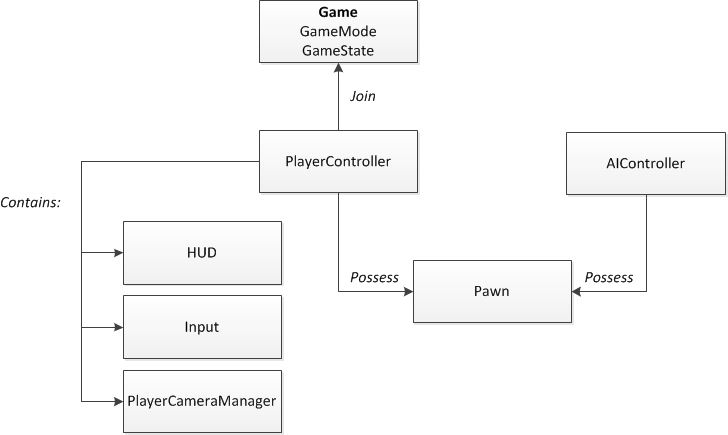
\includegraphics[width=1\textwidth]{figures/gameplay_chart.jpg}
	\caption{Diagram architektury rozgrywki}
	\label{fig-gameplay-chart}
\end{figure}

\chapter{Opis implementacji gry ,,thesis\_1``}

\section{Uruchomienie gry i podstawowe funkcje}
	\subsection{GameInfoInstance}

\section{System zapisu stanu}

\section{Postacie i zdolności}
	\subsection{BaseCharacter}
	\subsection{Skill}

\section{Networking}

\section{Animacje}
\chapter{Kolejny rozdział}

\begin{thebibliography}{9}

\bibitem{learning-unreal}
Joanna Lee, \textit{Learning Unreal Engine Game Development}, Packt Publishing, 2016

\bibitem{docs-ue4-features}
\textit{Engine Features}, \url{https://docs.unrealengine.com/latest/INT/Engine/index.html} (dostęp 30.12.2017)

\bibitem{docs-blueprints}
\textit{Blueprints Visual Scripting}, \url{https://docs.unrealengine.com/latest/INT/Engine/Blueprints/index.html} (dostęp 30.12.2017)

\bibitem{docs-gameplay-framework}
\textit{Gameplay Framework Quick Reference}, \url{https://docs.unrealengine.com/latest/INT/Gameplay/Framework/QuickReference/index.html} (dostęp 31.12.2017)

\bibitem{wiki-game-engine}
\textit{,,Game engine``, Wikipedia}, \url{https://en.wikipedia.org/wiki/Game_engine} {\mbox(dostęp 29.12.2017)}

\bibitem{unreal-wiki-replication}
\textit{Everything you ever wanted to know about replication (but were afraid to ask)}, \url{https://wiki.beyondunreal.com/Everything_you_ever_wanted_to_know_about_replication_\%28but_were_afraid_to_ask\%29#Function_call_replication_-_Sending_messages_between_server_and_client} (dostęp 30.12.2017)

\bibitem{nasdaq-video-games-industry}
Trevir Nath, \textit{Investing in Video Games: This Industry Pulls In More Revenue Than Movies, Music},
\url{http://www.nasdaq.com/article/investing-in-video-games-this-industry-pulls-in-more-revenue-than-movies-music-cm634585} {\mbox(dostęp 29.12.2017)}

\bibitem{the-human-race}
\textit{The Human Race – An Inside Look at the Technology Behind the Groundbreaking Real-Time Film from Epic Games, The Mill and Chevrolet}, \url{https://www.unrealengine.com/en-US/showcase/the-human-race-an-inside-look-at-the-technology-behind-the-groundbreaking-real-time-film-from-epic-games-the-mill-and-chevrolet} (dostęp 30.12.2017)

\bibitem{ikea-vr}
\textit{VIRTUAL REALITY - INTO THE MAGIC}, \url{http://www.ikea.com/ms/en_US/this-is-ikea/ikea-highlights/Virtual-reality/index.html} (dostęp 30.12.2017)

\end{thebibliography}

\beforelastpage

\end{document} 